\documentclass[12pt]{article}

\usepackage{amssymb,amsmath,amsfonts,eurosym,geometry,ulem,graphicx,caption,color,setspace,sectsty,comment,footmisc,caption,natbib,pdflscape,subfigure,array,hyperref}
\usepackage{booktabs}
\usepackage{multirow}
\usepackage{graphicx}
\usepackage{graphicx}
\usepackage{amsmath}
\usepackage{amsfonts}
\usepackage{amssymb}
\usepackage{tikz}
\usetikzlibrary{snakes}
\usepackage{float}
\usepackage{subfigmat}
\usepackage{etoolbox}
\usepackage{amssymb}
\usepackage{caption}
\usepackage{lscape}
\usepackage{graphicx}
\usepackage{pdflscape}
\usepackage{adjustbox}
\usepackage{xcolor}
\usepackage{graphicx}
\usepackage{hyperref}
\usepackage{hyperref}
\normalem

\onehalfspacing
\newtheorem{theorem}{Theorem}
\newtheorem{proposition}{Proposition}
\newenvironment{proof}[1][Proof]{\noindent\textbf{#1.} }{\ \rule{0.5em}{0.5em}}

\newtheorem{hyp}{Hypothesis}
\newtheorem{subhyp}{Hypothesis}[hyp]
\renewcommand{\thesubhyp}{\thehyp\alph{subhyp}}

\newcommand{\red}[1]{{\color{red} #1}}
\newcommand{\blue}[1]{{\color{blue} #1}}

\newcolumntype{L}[1]{>{\raggedright\let\newline\\arraybackslash\hspace{0pt}}m{#1}}
\newcolumntype{C}[1]{>{\centering\let\newline\\arraybackslash\hspace{0pt}}m{#1}}
\newcolumntype{R}[1]{>{\raggedleft\let\newline\\arraybackslash\hspace{0pt}}m{#1}}

\geometry{left=1.0in,right=1.0in,top=1.0in,bottom=1.0in}

\begin{document}

\begin{titlepage}
\title{GSF-3100 \\ Marchés des Capitaux \\ Gestion de portefeuille obligataire}
\date{\today}
\maketitle

\setcounter{page}{0}
\thispagestyle{empty}
\end{titlepage}
\pagebreak \newpage

\tableofcontents
\pagebreak \newpage

\section{Cadre de gestion de portefeuille obligataire}
Les quatre activités du processus de gestion des investissements:
\begin{enumerate}
\item Fixer les objectifs d'investissement (avec les contraintes associées)
\item Élaborer et mettre en œuvre une stratégie de portefeuille
\item Suivi du portefeuille
\item Ajustement du portefeuille.
\end{enumerate}

\section{Gestion obligataire par rapport à un indice du marché obligataire}
\subsection{Gestion passive}
Une stratégie de gestion passive suppose que les attentes du marché sont essentiellement correctes ou, plus précisément, que le gestionnaire n’a aucune raison d’être en désaccord avec ces attentes.  Peut-être parce qu’il n’a pas d’expertise particulière en matière de prévision. En définissant le profil de risque du portefeuille (par exemple, sensibilité aux taux d'intérêt et qualité de crédit) identique au profil de risque de l'indice de référence et en poursuivant une stratégie passive, le gestionnaire est tout à fait disposé à accepter un niveau de risque moyen (tel que défini par le risque de l'indice de référence) et un taux de rendement moyen (mesuré par le rendement de l'indice de référence et du portefeuille). Dans le cadre d'une stratégie passive, le gestionnaire n'a pas à faire de prévisions indépendantes et le portefeuille devrait suivre de très près l'indice de référence.
\subsection{Gestion active}
Une stratégie de gestion active repose essentiellement sur la capacité de prévision du gestionnaire. Les gestionnaires actifs estiment qu'ils possèdent des compétences supérieures en matière de prévision des taux d'intérêt, d'évaluation du crédit ou dans un autre domaine qui peut être utilisé pour exploiter les opportunités du marché. Le rendement du portefeuille devrait augmenter si les prévisions du gestionnaire de l’évolution future des facteurs qui influent sur les rendements des titres à revenu fixe (par exemple, les variations des taux d’intérêt ou des écarts de crédit) sont plus précises que celles reflétées dans les prix actuels des titres à revenu fixe.  Le gestionnaire peut créer de petits décalages (amélioration) ou de grands décalages (gestion active à part entière) par rapport au benchmark pour profiter de cette expertise.

\section{Classification des stratégies}

\subsection{Indexation d'obligations pure (ou approche de réplication complète)}
L'objectif ici est de produire un portefeuille parfaitement adapté au portefeuille de référence. L'approche d'indexation purement obligataire tente de dupliquer l'indice en détenant toutes les obligations de l'indice dans le même pourcentage que l'indice. La réplication complète est généralement très difficile et coûteuse à mettre en œuvre dans le cas des indices obligataires. De nombreuses émissions dans un indice obligataire typique (en particulier les non-bons du Trésor) sont assez illiquides et très rarement négociées. Pour cette raison, la réplication complète d'un indice obligataire est rarement tentée en raison de la difficulté, de l'inefficacité et du coût élevé de mise en œuvre.
\subsection{Indexation améliorée en faisant correspondre les principaux facteurs de risque}
Ce style de gestion utilise une approche d'échantillonnage dans le but de faire correspondre les principaux facteurs de risque de l'indice et d'obtenir un rendement supérieur à celui d'une réplication complète. Les principaux facteurs de risque sont généralement des influences majeures sur le prix des obligations, telles que les variations du niveau des taux d'intérêt, les torsions de la courbe des taux et les variations de l'écart entre les bons du Trésor et les non-bons du Trésor. 
\begin{enumerate}
\item En investissant dans un échantillon d'obligations plutôt que dans l'ensemble de l'indice, le gestionnaire réduit les coûts de construction et d'entretien du portefeuille. Même si une approche d'échantillonnage suivra généralement l'indice de moins près que la réplication complète, on s'attend à ce que cet inconvénient soit plus que compensé par la baisse des dépenses.
\item En faisant correspondre les principaux facteurs de risque, le portefeuille est affecté par des événements de grande ampleur sur le marché au même degré que l'indice de référence. Le gestionnaire de portefeuille peut essayer d’améliorer le rendement du portefeuille en utilisant des obligations qui sont perçues comme sous-évaluées, par exemple.
\end{enumerate}
\subsection{Indexation améliorée grâce à de petites incohérences de facteurs de risque}
Tout en faisant correspondre la duration (sensibilité aux taux d'intérêt), ce style permet au gestionnaire de faire pencher le portefeuille en faveur de l'un des autres facteurs de risque. Le gestionnaire peut essayer d'augmenter légèrement le rendement en recherchant la valeur relative dans certains secteurs, la qualité, la structure des termes, etc. Les décalages sont faibles
et visent simplement à améliorer suffisamment le rendement du portefeuille pour surmonter la différence de coûts administratifs entre le portefeuille et l’indice.
\subsection{Gestion active par des inadéquations plus importantes des facteurs de risque}
Le gestionnaire de portefeuille recherche maintenant activement les occasions sur le marché d'augmenter le rendement. Le gestionnaire peut surpondérer les obligations notées A par rapport aux obligations notées AA / Aaa, surpondérer les entreprises par rapport aux bons du Trésor. L’objectif du gestionnaire est de produire des rendements suffisants pour surmonter les coûts de transaction supplémentaires de ce style tout en maîtrisant le risque.
\subsection{Gestion active à part entière}
Une gestion active à part entière implique la possibilité d'inadéquations agressives sur la durée, les pondérations sectorielles et d'autres facteurs.

\section{Sélection d'un indice obligataire de référence: considérations générales}
Une fois la décision d'indexation prise, d'importantes questions de suivi demeurent:
\begin{itemize}
\item Quel indice de référence dois-je choisir?
\item L'indice de référence doit-il avoir une durée courte ou une durée longue?
\item La qualité de crédit de l’indice de référence est-elle adaptée au rôle que le portefeuille obligataire jouera dans mon portefeuille global?
\item Au risque de simplifier à l'extrême, vous devriez choisir l'indice contenant des caractéristiques qui correspondent étroitement aux caractéristiques souhaitées de votre portefeuille.
\end{itemize}
Le choix dépend fortement de quatre facteurs:
\subsection{Risque de valeur marchande}
Le risque de valeur de marché du portefeuille et de l'indice de référence doit être comparable. Étant donné une courbe de rendement normale à pente ascendante, le rendement à l'échéance d'un portefeuille d'obligations augmente à mesure que la maturité du portefeuille augmente. À mesure que la maturité et la durée d'un portefeuille augmentent, le risque de marché augmente. Pour les investisseurs averses au risque, l'indice à court ou à moyen terme peut être plus approprié comme indice de référence que l'indice long.
\subsection{Risque de revenu}
Le portefeuille et l'indice de référence devraient fournir des flux de revenus garantis comparables. De nombreux investisseurs (par exemple, les fondations et les retraités) préfèrent les portefeuilles qui génèrent un niveau de revenu élevé tout en conservant le capital. Investir dans un portefeuille long terme peut garantir un flux de revenu fiable sur une longue période et ne soumet pas le flux de revenu aux caprices de la fluctuation des taux d'intérêt. Si la stabilité et la fiabilité des revenus sont les principaux besoins de l'investisseur, alors le portefeuille long terme est le moins risqué et le portefeuille court terme est le plus risqué.
\subsection{Le risque de crédit}
Le risque de crédit moyen de l’indice de référence doit être adapté au rôle du portefeuille indexé dans le portefeuille global de l’investisseur et satisfaire à toute contrainte imposée à la qualité du crédit dans la déclaration de politique d’investissement de l’investisseur. La diversification des émetteurs de l'indice de référence devrait également être satisfaisante pour l'investisseur.
\subsection{Le risque de responsabilité des passifs}
Ce risque doit être minimisé.  En général, il est prudent de faire correspondre les caractéristiques d'investissement (par exemple, la durée) des actifs et des passifs, si les passifs jouent un rôle. Le choix d'un indice de référence approprié doit refléter la nature du passif: les investisseurs ayant des engagements à long terme devraient choisir un indice long terme.  Bien sûr, les investisseurs obligataires qui n'ont pas de passifs ont beaucoup plus de latitude dans le choix d'un indice de référence en raison de l'absence de cette restriction.
\section{Suivi des risques}
Le risque de suivi (également appelé tracking error) est une mesure de la variabilité avec laquelle le rendement d'un portefeuille suit le rendement d'un indice de référence. Plus précisément, le risque de suivi est défini comme l'écart type du rendement actif du portefeuille, où le rendement actif pour chaque période est défini comme
\begin{align*}
AR = PR-BIR
\end{align*}
\begin{itemize}
\item $AR=$ Rendement actif 
\item $PR=$ Rendement du portefeuille 
\item $BIR=$ Rendement de l'indice de référence
\end{itemize}
Par conséquent
\begin{align*}
TR=\sigma_{AR}
\end{align*}
\begin{itemize}
\item $TR=$ Tracking error
\item $\sigma_{AR}=$ Écart type des rendements actifs
\end{itemize}
\section{Stratégies d'indexation améliorées}
Bien qu'il y ait des dépenses et des coûts de transaction associés à la construction et au rééquilibrage d'un portefeuille indexé, il n'y a pas de coûts similaires pour l'indice lui-même (car il s'agit en fait d'un portefeuille papier). Par conséquent, il est raisonnable de s'attendre à ce qu'un portefeuille parfaitement indexé sous-performe l'indice du montant de ces coûts. Pour cette raison, le gestionnaire d’obligations peut choisir de récupérer ces coûts en cherchant à améliorer le rendement du portefeuille.  Voici un certain nombre de façons (c'est-à-dire des stratégies d'amélioration de l'indice) dans lesquelles cela peut être fait: 
\subsection{Améliorations à moindre coût}
Les gestionnaires peuvent augmenter le rendement net du portefeuille en maintenant simplement des contrôles stricts sur les frais de négociation et les frais de gestion. Bien que relativement faibles, les dépenses varient considérablement d'un fonds indiciel à l'autre. Lorsque des gestionnaires externes sont embauchés, le promoteur du régime peut exiger que les gestionnaires soumettent à nouveau leurs frais de gestion tous les deux ou trois ans pour s'assurer que ces frais restent aussi bas que possible.
\subsection{Améliorations de la sélection des problèmes}
Le gestionnaire peut identifier et sélectionner des titres sous-évalués sur le marché, par rapport à la valeur théorique d’un modèle d’évaluation. De nombreux gérants mènent leur propre analyse de crédit plutôt que de se fier uniquement aux notations fournies par les sociétés de notation obligataire. En conséquence, le gestionnaire peut être en mesure de sélectionner les problèmes qui seront bientôt mis à niveau et d'éviter les problèmes qui sont sur le point d'être rétrogradés.
\subsection{Positionnement de la courbe des rendement}
Certaines échéances le long de la courbe des taux ont tendance à rester constamment surévaluées ou sous-évaluées. Par exemple, la courbe des taux a souvent une pente négative entre 25 et 30 ans, même si le reste de la courbe peut avoir une pente positive. Ces obligations à long terme ont tendance à être des placements populaires pour de nombreuses institutions, ce qui se traduit par un prix surévalué par rapport aux obligations de maturité plus courte. En surpondérant les zones sous-évaluées de la courbe et en sous-pondérant les zones surévaluées, le gestionnaire peut être en mesure d’améliorer le rendement du portefeuille.
\subsection{Positionnement sectoriel et qualité}
Cette technique d'amélioration du rendemen prend deux formes:
\begin{enumerate}
\item Maintien d'une inclinaison de rendement vers les entreprises de courte durée. L'expérience a montré que le meilleur écart de rendement par unité de risque de duration est généralement disponible dans les titres de sociétés dont l'échéance est inférieure à cinq ans (c.-à-d. Les sociétés à découvert). Un gestionnaire peut augmenter le rendement du portefeuille sans augmentation proportionnelle du risque en orientant le portefeuille vers ces titres. La stratégie n'est pas sans risques, même si ceux-ci sont gérables. Le risque de défaut est plus élevé pour les titres de sociétés, mais ce risque peut être géré grâce à une diversification appropriée. (Le risque de défaut est le risque de perte si un émetteur ou une contrepartie ne remplit pas ses obligations contractuelles.)
\item Sur- ou sous-pondération périodique des secteurs (par exemple, bons du Trésor vs entreprises) ou des qualités. Conduit à petite échelle, le gestionnaire peut surpondérer les bons du Trésor lorsque les écarts devraient s'élargir (par exemple, avant une récession) et les sous-pondérer lorsque les écarts devraient se resserrer. Bien que cette stratégie présente certaines similitudes avec la gestion active, elle est mise en œuvre à une si petite échelle que l'objectif est de gagner suffisamment de rendement supplémentaire pour compenser certaines des dépenses d'indexation, et non de surperformer l'indice par une large marge comme c'est le cas en actif la gestion.
\end{enumerate}
\subsection{Positionnement par rapport au risque d'appel}
Une baisse des taux d'intérêt entraînera inévitablement le retrait anticipé de certaines obligations remboursables par appel. À mesure que les taux baissent, l'investisseur doit déterminer la probabilité que l'obligation soit appelée.  Il existe un point de croisement auquel l'investisseur moyen ne sait pas si l'obligation est susceptible d'être appelé. Près de ce point, la performance réelle d'une obligation peut être sensiblement différente de ce à quoi on pourrait s'attendre, compte tenu de la duration effective de l'obligation (duration ajustée pour tenir compte des options incorporées) la sensibilité réelle au prix a tendance à être inférieure à celle prédite par la durée effective des obligations. Une baisse des rendements entraînera une sous-performance par rapport à la prédiction du modèle de durée effective. Cette sous-performance crée une opportunité pour le gestionnaire de portefeuille de sous-pondérer ces émissions dans ces conditions.

\section{Activités supplémentaires requises pour le gestionnaire actif}
Les gestionnaires actifs ont un ensemble d'activités qu'ils doivent mettre en œuvre auxquelles les gestionnaires passifs ne sont pas confrontés. Après avoir sélectionné le type de stratégie active à poursuivre, le gestionnaire actif:

\subsection{Identifiez les discordances d'index à exploiter}
Le choix des inadéquations est généralement basé sur l'expertise du gestionnaire. Si la force du gestionnaire réside dans la prévision des taux d’intérêt, des décalages délibérés de durée seront créés entre le portefeuille et l’indice de référence. Si le gérant possède des compétences supérieures pour identifier les titres sous-évalués ou les secteurs sous-évalués, les asymétries sectorielles seront poursuivies.
\subsection{Extrapolez les attentes du marché à partir des données du marché}
Comme indiqué précédemment, les prix actuels du marché sont le résultat de l'application de leur jugement par tous les investisseurs aux obligations individuelles. En analysant ces prix et rendements, des données supplémentaires peuvent être obtenues. Par exemple, les taux à terme peuvent être calculés à partir des points le long de la courbe de rendement des taux au comptant. Ces taux à terme peuvent donner un aperçu de la direction et du niveau que les investisseurs pensent que les taux seront dirigés à l'avenir.
\subsection{Prévoyez indépendamment les intrants nécessaires et comparez-les aux attentes du marché}
Après avoir calculé les taux à terme, le gestionnaire actif peut croire avec ferveur que ces taux sont trop élevés et que les taux d'intérêt futurs n'atteindront pas ces niveaux. Après avoir comparé sa prévision de taux à terme avec celle d'autres investisseurs, le gestionnaire peut décider de créer un décalage de durée. En augmentant la durée du portefeuille, le gestionnaire peut profiter (s’il a raison) de la baisse de la courbe des taux qui en résulte, car d’autres investisseurs se rendent compte finalement que leur prévision était incorrecte.
\subsection{Estimer les valeurs relatives des titres afin d'identifier les zones de sous-évaluation ou de surévaluation}
Encore une fois, l'accent dépend de l'ensemble des compétences du gestionnaire. Certains gérants feront des décalages de duration tandis que d'autres se concentreront sur les titres sous-évalués. Dans tous les cas, cependant, les managers appliqueront leurs compétences pour essayer d'exploiter les opportunités au fur et à mesure qu'elles se présentent.
\section{Analyse du rendement total et analyse des scénarios}
Avant d’exécuter une transaction, un gestionnaire actif doit évidemment analyser l’impact de la transaction sur le rendement du portefeuille. Quels outils le gestionnaire a-t-il dans sa trousse à outils pour aider à évaluer les caractéristiques de risque et de rendement d'une transaction? Les deux principaux outils sont l'analyse du rendement total et l'analyse de scénarios.
\subsection{Le rendement total d’une obligation}
Le rendement total d’une obligation est le taux de rendement qui équivaut à la valeur future des flux de trésorerie de l’obligation avec le prix total de l’obligation. En tant que tel, le rendement total prend en compte les trois sources de rendement potentiel: le revenu du coupon, le revenu de réinvestissement et la variation du prix. 
\subsection{L’analyse du rendement total}
L’analyse du rendement total consiste à évaluer l’effet attendu d’une transaction sur le rendement total du portefeuille en fonction d’une prévision de taux d’intérêt.

\section{Gérer les fonds contre les passifs}
Nous tournons maintenant notre attention vers la gestion des fonds par rapport à un passif ou un ensemble de passifs.
\subsection{Stratégies de dévouement}
Les stratégies de dévouement sont des stratégies spécialisées de gestion de portefeuille contenant des titres à revenu fixe conçues pour répondre aux besoins de financement spécifiques de l'investisseur. Ils sont généralement classés comme passifs par nature, bien qu'il soit possible d'y ajouter des éléments de gestion active.  L'immunisation est un type important de stratégie de dévouement. L'immunisation vise à construire un portefeuille qui, sur un horizon spécifié, rapportera un rendement prédéterminé indépendamment des variations des taux d'intérêt. Une autre stratégie de dévouement largement utilisée est l'appariement des flux de trésorerie, qui fournit le financement futur d'un flux de passif à partir du coupon et des remboursements de principal échus du portefeuille.

\begin{table}[H]
\caption{Quatre types (ou classes) types de passifs}
\begin{tabular}{@{}ccl@{}}
\toprule
\textbf{Montant (\$)} & \textbf{Moment (date)} & \multicolumn{1}{c}{\textbf{Exemple}}            \\ \midrule
Connu                 & Connu                  & Un remboursement du principal                   \\
Connu                 & Inconnu                & Un versement d'assurance-vie                    \\
Inconnu               & Connu                  & Un versement de rente à taux variable           \\
Inconnu               & Inconnu                & Prestations de soins de santé après la retraite \\ \bottomrule
\end{tabular}
\end{table}
Plus les passifs sont incertains, plus il devient difficile d’utiliser une stratégie de dévouement passif pour atteindre les objectifs du portefeuille. Pour cette raison, à mesure que les passifs deviennent plus incertains, les gérants insèrent souvent des éléments de gestion active. Le but de cette action est d'augmenter le potentiel de hausse du portefeuille tout en garantissant simultanément un ensemble de flux de trésorerie qui devraient être adéquats pour payer les passifs anticipés.

\section{Stratégies d'immunisation}
L'immunisation est une stratégie populaire pour \textbf{verrouiller} un taux de rendement garanti sur un horizon temporel particulier. À mesure que les taux d'intérêt augmentent, la baisse du prix d'un titre à revenu fixe est généralement au moins partiellement compensée par un montant plus élevé de revenu de réinvestissement. À mesure que les taux baissent, l’augmentation du prix d’un titre est généralement au moins partiellement compensée par une baisse du revenu de réinvestissement.

\vspace{0.5cm}

Pour un horizon temporel arbitraire, les effets prix et réinvestissement ne se compensent généralement pas exactement: \textbf{la variation de prix peut être supérieure ou inférieure à la variation des revenus de réinvestissement}.  Le but de l'immunisation est d'identifier le portefeuille pour lequel la variation de prix est exactement égale à la variation des revenus de réinvestissement à l'horizon temporel d'intérêt. Si le gestionnaire peut construire un tel portefeuille, un taux de rendement assuré sur cet horizon est verrouillé.
\subsection{Immunisation classique à période unique}
L'immunisation classique peut être définie comme la création d'un portefeuille à revenu fixe qui produit un rendement assuré pour un horizon temporel spécifique, indépendamment de tout déplacement parallèle de la courbe de rendement. Dans sa forme la plus élémentaire, les caractéristiques importantes de l'immunisation sont :
\begin{enumerate}
\item Horizon temporel spécifié.
\item Taux de rendement assuré pendant la période de détention jusqu'à une date d'horizon fixe.
\item Isolation contre les effets des variations de taux d'intérêt sur la valeur du portefeuille à la date d'horizon.
\end{enumerate}
Le mécanisme fondamental de l'immunisation est une structure de portefeuille qui équilibre la variation de la valeur du portefeuille à la fin de l'horizon d'investissement avec le rendement du réinvestissement des flux de trésorerie du portefeuille (paiements de coupons et titres arrivant à échéance). 

\vspace{0.5cm}

L'immunisation nécessite de compenser le risque de prix et le risque de réinvestissement. Pour réaliser cet équilibrage, il faut gérer la durée.  Le fait de fixer la duration du portefeuille à l'horizon temporel spécifié du portefeuille garantit la compensation des sources de rendement différentiel positives et négatives sous certaines hypothèses, y compris l'hypothèse que le portefeuille immunisant a la même valeur actuelle que le passif à immuniser

\vspace{0.5cm}
Gardez à l'esprit que pour immuniser la valeur cible ou le rendement cible d'un portefeuille contre une variation du rendement du marché, un gestionnaire doit investir dans une obligation ou un portefeuille obligataire dont
\begin{enumerate}
\item la durée est égale à l'horizon d'investissement.
\item la valeur actuelle initiale de tous les flux de trésorerie correspondent à la valeur actuelle du passif futur.
\end{enumerate}

\section{Rééquilibrer un portefeuille immunisé}
le rendement du marché fluctuera sur l'horizon d'investissement. En conséquence, la durée du portefeuille changera à mesure que le rendement du marché évoluera. La durée changera également simplement en raison du passage du temps. Dans tout environnement de taux d'intérêt différent d'une structure de terme fixe, la durée d'un portefeuille changera à un taux différent dans le temps. 

\vspace{0.5cm}

\textbf{À quelle fréquence un portefeuille doit-il être rééquilibré pour ajuster sa durée?}

\vspace{0.5cm}

La réponse consiste à équilibrer les coûts et les avantages du rééquilibrage.
\begin{itemize}
\item Un rééquilibrage plus fréquent augmente les coûts de transaction, réduisant ainsi la probabilité d'atteindre le rendement cible.
\item Un rééquilibrage moins fréquent fait que la durée s'écarte de la durée cible, ce qui réduit également la probabilité d'atteindre le rendement cible
\end{itemize}
le gestionnaire est confronté à un compromis: \textbf{certains coûts de transaction doivent être acceptés pour éviter que la durée ne s'éloigne trop de son objectif, mais une certaine inadéquation de la durée doit être vécue, sinon les coûts de transaction deviendront prohibitifs}.

\section{Détermination du rendement cible}
Compte tenu de la structure par terme des taux d'intérêt ou de la courbe de rendement prévalant au début de la période d'horizon, le taux de rendement assuré de l'immunisation peut être déterminé. Théoriquement, ce taux de rendement cible de l'immunisation est défini comme le rendement total du portefeuille, en supposant qu'il n'y ait pas de changement dans la structure par terme.  Ce taux de rendement cible différera toujours du rendement actuel du portefeuille à l'échéance, sauf si la structure par terme est plate (ni croissante ni décroissante), car en raison du passage du temps.

\vspace{0.5cm}

Autrement dit, pour une courbe de rendement à pente ascendante, le rendement à l'échéance d'un portefeuille peut être très différent de son taux de rendement cible d'immunisation tandis que, pour une courbe de rendement plate, le rendement à l'échéance se rapprocherait à peu près du rendement cible assuré.

\vspace{0.5cm}

En général, pour une courbe de rendement à pente ascendante, le taux de rendement cible de l'immunisation sera inférieur au rendement à l'échéance en raison du rendement de réinvestissement plus faible. À l'inverse, une courbe de rendement négative ou descendante se traduira par un taux de rendement cible d'immunisation supérieur au rendement à l'échéance en raison du rendement de réinvestissement plus élevé.

\vspace{0.5cm}

Les mesures alternatives du taux de rendement cible de l'immunisation comprennent le rendement impliqué par une obligation à coupon zéro de qualité et de durée comparables à celles du portefeuille obligataire et une estimation basée sur les résultats d'une simulation qui rééquilibre le portefeuille initial, compte tenu des scénarios de variation des taux d'intérêt. .

\section{Extensions de la théorie classique de l'immunisation}
La théorie classique de la vaccination repose sur plusieurs hypothèses:
\begin{enumerate}
\item Tout changement de la courbe de rendement est un changement parallèle, c'est-à-dire que les taux d'intérêt augmentent ou diminuent du même montant pour toutes les échéances.
\item Le portefeuille est évalué à une date d'horizon fixe et il n'y a pas d'entrées ou de sorties de trésorerie intermédiaires avant la date d'horizon.
\item La valeur cible de l'investissement est définie comme la valeur du portefeuille à la date de l'horizon si la structure des taux d'intérêt ne change pas (c'est-à-dire qu'il n'y a pas de changement des taux à terme).
\end{enumerate}

\begin{figure}[H]
\caption{Changements de la valeur du portefeuille causés par des changements parallèles de taux d'intérêt pour un portefeuille immunisé.}
\centering
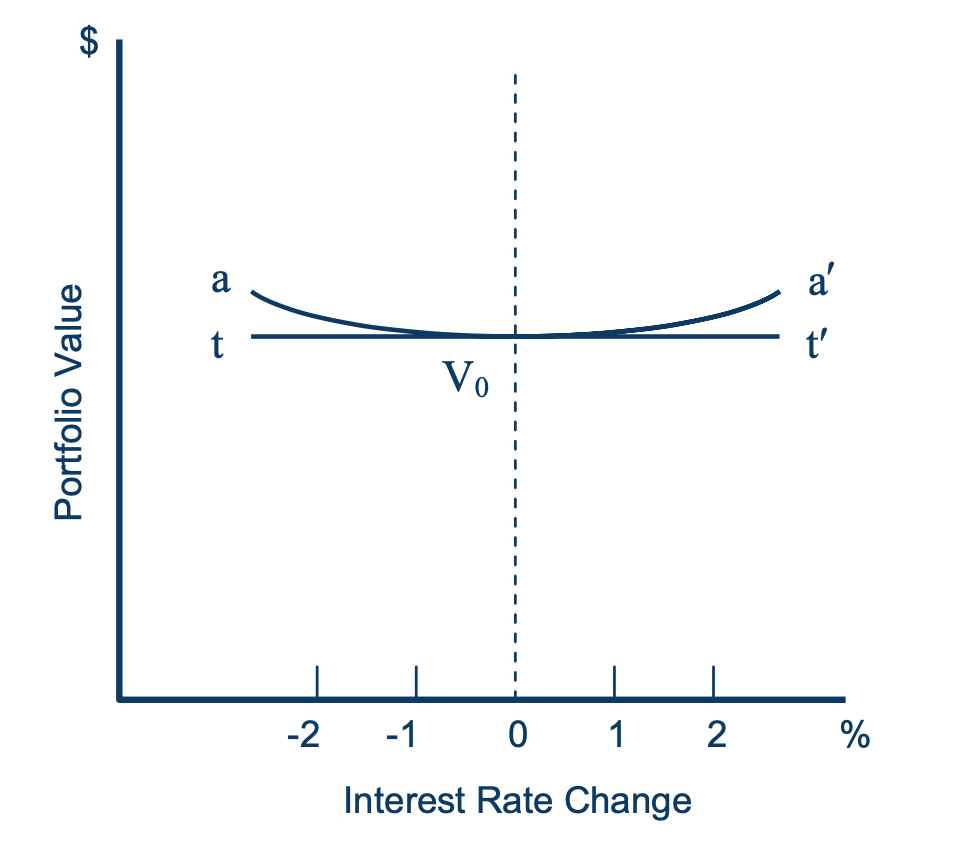
\includegraphics[width=12cm]{1}
\end{figure}

\begin{figure}[H]
\caption{Deux possibilités de changements de la valeur du portefeuille causés par des variations non parallèles des taux d'intérêt pour un portefeuille immunisé.}
\centering
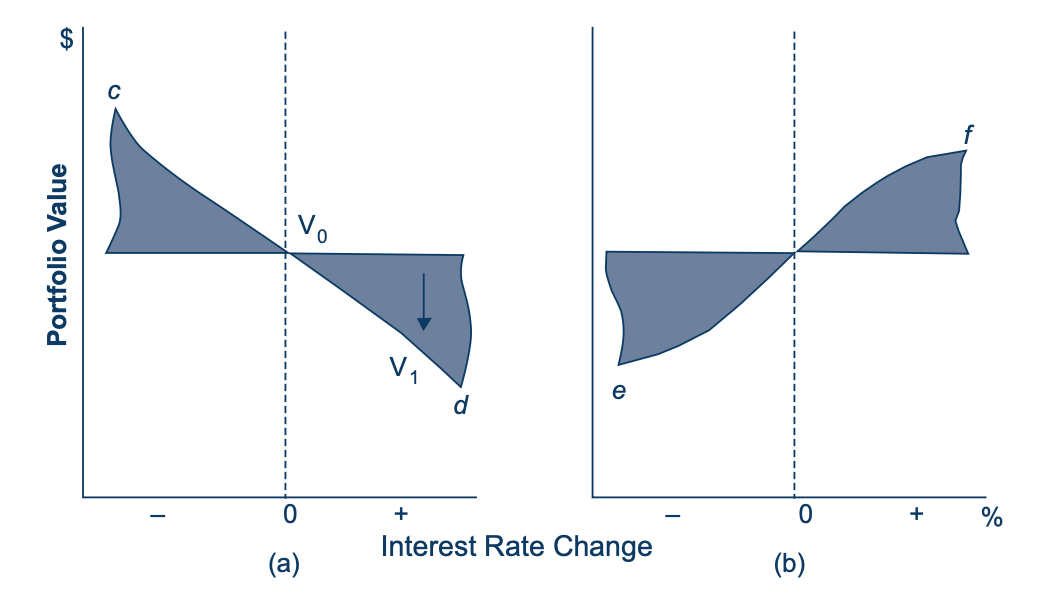
\includegraphics[width=14cm]{2}
\end{figure}

La figure 1 illustre la nature de la valeur du portefeuille, compte tenu d'un portefeuille immunisé et des variations parallèles des taux. La courbe $a-a^'$ représente le comportement de la valeur du portefeuille pour divers changements de taux, allant d'une baisse à une augmentation comme indiqué sur l'axe horizontal. Le point $V_0$ de la ligne $t-t^'$ est le niveau de la valeur du portefeuille en supposant l'absence de changement des taux.  Un portefeuille immunisé soumis à des déplacements parallèles de la courbe des taux fournira une valeur de portefeuille au moins aussi élevée à la date d'horizon que la valeur cible assurée, qui devient ainsi la valeur minimale. Par conséquent, si les hypothèses de la théorie classique sont valables, l'immunisation fournit une stratégie à risque minimum.

\vspace{0.5cm}


La figure 2 illustre la relation entre la valeur d'un portefeuille immunisé de façon classique et les variations des taux d'intérêt lorsque les taux d'intérêt ne changent pas de façon parallèle.  Selon la forme du décalage non parallèle, la relation indiquée en $a)$ ou celle illustrée en $b)$ se produira. Cette figure montre la possibilité (dans les cas $d$ et $e$) que la valeur d'un portefeuille immunisé de manière classique puisse être inférieure à la cible. Le point important est que le simple fait de faire correspondre la durée du portefeuille à l'horizon d'investissement comme condition d'immunisation ne peut pas empêcher des écarts importants par rapport à la valeur cible.

\vspace{0.5cm}

Une extension naturelle de la théorie classique de l'immunisation est d'étendre la théorie au cas de variations non parallèles des taux d'intérêt. Deux approches ont été adoptées.

\begin{enumerate}
\item La première approche a consisté à modifier la définition de la duration afin de permettre des changements non parallèles de la courbe des taux, tels que la duration multifonctionnelle (également appelée duration fonctionnelle ou duration des taux directeurs)
\item La deuxième approche est une stratégie qui peut gérer tout changement arbitraire de taux d'intérêt de sorte qu'il n'est pas nécessaire de spécifier une autre mesure de durée. Cette approche, développée par Fong et Vasicek (1984), établit une mesure du risque d'immunisation contre toute variation arbitraire des taux d'intérêt. La mesure du risque d'immunisation peut alors être minimisée sous réserve que la durée du portefeuille soit égale à l'horizon d'investissement, ce qui se traduit par un portefeuille avec une exposition minimale aux fluctuations des taux d'intérêt.
\end{enumerate}

\vspace{0.5cm}

Une deuxième extension de la théorie classique d'immunisation s'applique au dépassement des limites d'un horizon fixe (la deuxième hypothèse dont dépend l'immunisation). Marshall et Yawitz (1982) ont démontré que, dans l'hypothèse de variations parallèles des taux d'intérêt, une borne inférieure existe sur la valeur d'un portefeuille d'investissement à un moment donné, bien que cette borne inférieure puisse être inférieure à la valeur réalisée si les taux d'intérêt ne changent pas. Fong et Vasicek (1984) et Bierwag, Kaufman et Toevs (1979) ont étendu l'immunisation au cas des responsabilités multiples. L'immunisation à responsabilité multiple implique une stratégie d'investissement qui garantit le respect d'un calendrier spécifié de passifs futurs, quel que soit le type de changement dans les variations des taux d'intérêt. Fong et Vasicek (1984) ont fourni une généralisation de la mesure du risque d'immunisation pour le cas de responsabilité multiple.

\vspace{0.5cm}

La troisième extension de la théorie classique de l'immunisation consiste à analyser le compromis entre le risque et le rendement des portefeuilles immunisés. Fong et Vasicek (1983) ont montré comment ce compromis peut être analysé. Leur approche est appelée \textbf{maximisation du rendement}.

\vspace{0.5cm}

La quatrième extension de la théorie classique de l'immunisation consiste à intégrer des stratégies d'immunisation à des éléments de stratégies de gestion active de portefeuille obligataire. L'objectif traditionnel de l'immunisation a été la protection contre les risques, avec peu de considération pour les retours possibles. Leibowitz et Weinberger (1981) ont proposé une technique appelée immunisation contingente, qui offre une certaine souplesse dans la poursuite de stratégies actives tout en garantissant un certain rendement minimum dans le cas d'un changement de taux parallèle. Dans l'immunisation contingente, l'immunisation sert de stratégie de repli si le portefeuille géré activement ne croît pas à un certain rythme.

\section{Durée et convexité des actifs et des passifs}
Pour qu'un gestionnaire puisse avoir une image claire de l'excédent économique du portefeuille - défini comme la valeur marchande des actifs moins la valeur actuelle des passifs - la durée et la convexité des actifs et des passifs doivent être comprises. Se concentrer uniquement sur la durée des actifs d’une entreprise ne donnera pas une véritable indication du risque de taux d’intérêt total pour une entreprise.
\section{Types de risque}
À mesure que l'environnement de marché évolue, le gestionnaire de portefeuille court le risque de ne pas être en mesure de payer les dettes à leur échéance. Les trois sources de ce risque sont le risque de taux d'intérêt, le risque de réclamation conditionnelle et le risque de plafonnement.
\begin{enumerate}
\item \textbf{Risque de taux d'intérêt}: Étant donné que les prix de la plupart des titres à revenu fixe évoluent à l'opposé des taux d'intérêt, une hausse des taux d'intérêt aura une incidence défavorable sur la valeur d'un portefeuille. Si des actifs doivent être vendus pour assurer le service des passifs, le gestionnaire peut trouver un manque à gagner. Le risque de taux d'intérêt est le plus grand risque auquel un gestionnaire de portefeuille sera confronté.
\item \textbf{Risque de réclamations éventuelles}: Lorsqu'un titre comporte une disposition de réclamation conditionnelle, explicite ou implicite, il existe un risque associé. Dans un environnement de taux en baisse, le gestionnaire peut interrompre les paiements de coupons lucratifs et recevoir le principal (comme c'est le cas avec les titres adossés à des créances hypothécaires lorsque les prêts hypothécaires sous-jacents remboursent le principal).La perte des coupons est déjà assez grave, mais maintenant le principal doit être réinvesti à un taux inférieur. De plus, la valeur marchande d'un titre appelable se stabilisera au prix d'appel, plutôt que de continuer à augmenter comme le ferait un titre non remboursable.
\item \textbf{Risque de plafond}: Un actif qui effectue des paiements à taux variable aura généralement des plafonds associés au taux variable. Le gérant risque de voir le niveau des taux du marché augmenter alors que les rendements des actifs sont plafonnés. Cet événement peut affecter gravement la valeur des actifs.
\end{enumerate}

\section{Minimisation des risques pour les portefeuilles immunisés}
\begin{figure}[H]
\caption{Illustration de la mesure des risques liés à l'immunisation}
\centering
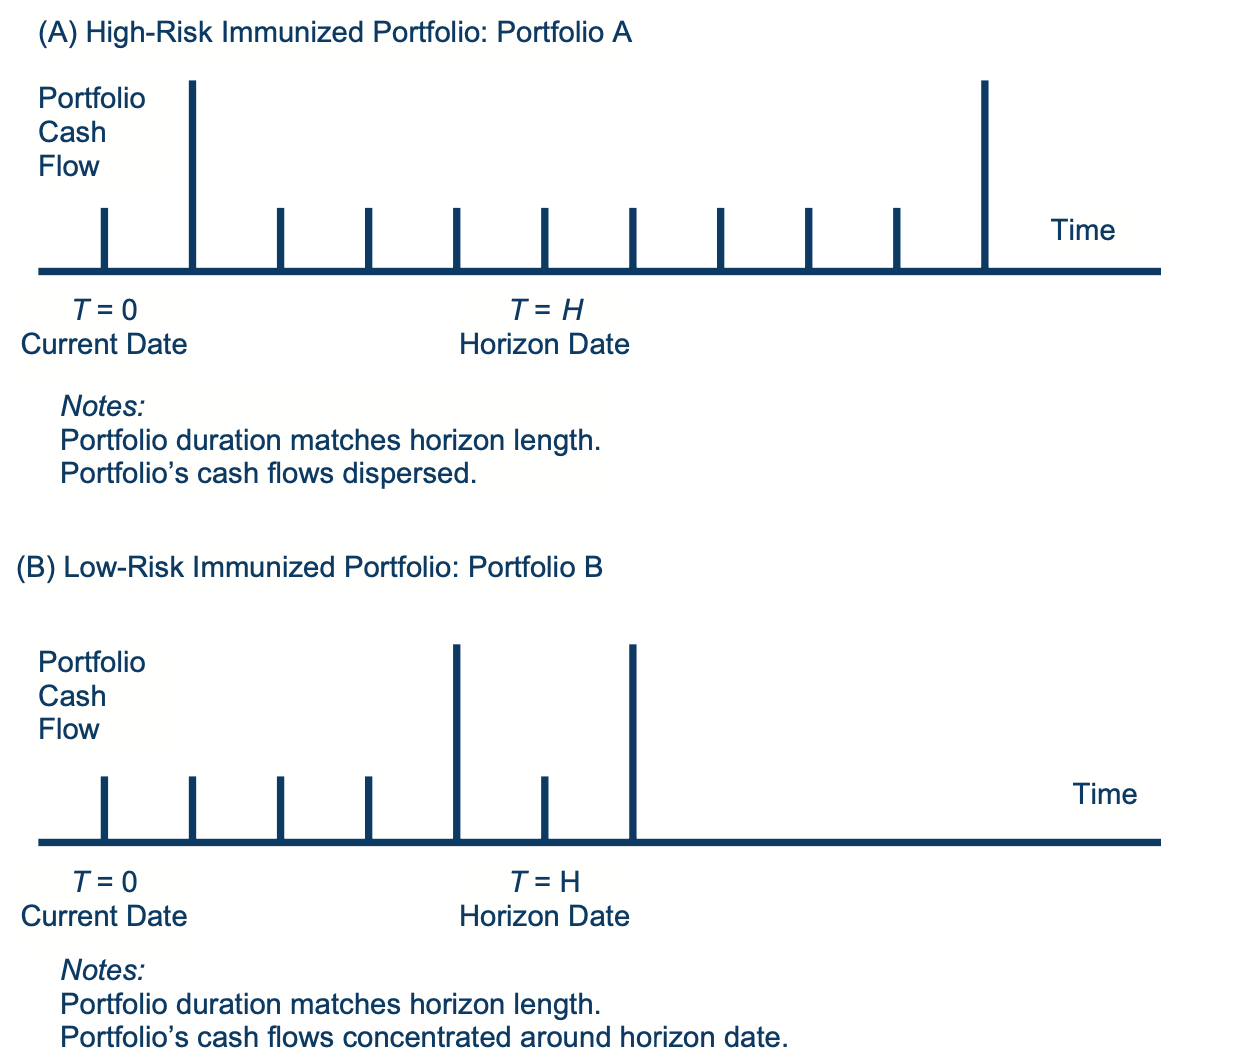
\includegraphics[width=14cm]{3}
\end{figure}

Dans la figure 3, les pics représentent les flux de trésorerie réels du portefeuille. Les pics les plus élevés représentent les flux de trésorerie réels générés par les titres à l'échéance, tandis que les pics plus petits représentent les paiements de coupons. Le portefeuille A et le portefeuille B sont tous deux composés de deux obligations dont la durée est égale à l'horizon d'investissement. Le portefeuille A est, en fait, un portefeuille haltère (un portefeuille composé d'échéances courtes et longues par rapport à la date d'horizon et des paiements de coupons intermédiaires). Le portefeuille B, cependant, est un portefeuille de bullet (les échéances des obligations sont très proches de l'horizon d'investissement). Si les deux portefeuilles ont des durées égales à la longueur de l'horizon, les deux portefeuilles sont immunisés contre des variations de taux parallèles. Cependant, lorsque les taux d'intérêt changent de manière arbitraire et non parallèle, l'effet sur la valeur des deux portefeuilles diffère )(le portefeuille haltères est plus risqué que le portefeuille bullet).

\vspace{0.5cm}

Si les taux courts terme baissent tandis que les taux longs terme augmentent :
\begin{itemize}
\item Les portefeuilles haltères et bullet réaliseraient une baisse de la valeur du portefeuille à la fin de l'horizon de placement sous la valeur de placement cible, car ils subiraient une perte en capital en plus de taux de réinvestissement plus faibles.
\item La baisse serait toutefois nettement plus élevée pour le portefeuille d'haltères
\begin{itemize}
\item Le portefeuille d'haltères connaît des taux de réinvestissement plus bas plus longtemps que le portefeuille de bullet
\item Une plus grande partie du portefeuille haltères est toujours en souffrance à la fin de l'horizon de placement, ce qui signifie que la même augmentation de taux entraîne beaucoup plus de perte en capital.
\end{itemize}
En bref, le portefeuille bullet est moins exposé aux variations de la structure des taux d'intérêt que le portefeuille haltères.

\section{Stratégies d'appariement des flux de trésorerie}
L'appariement des flux de trésorerie est une alternative à l'immunisation de responsabilité multiple dans la gestion actif / passif. L'appariement des flux de trésorerie est une stratégie attrayante car le gestionnaire de portefeuille n'a besoin que de sélectionner des titres qui correspondent au moment et au montant des passifs. Conceptuellement, une obligation est sélectionnée avec une échéance qui correspond au dernier passif, et un montant de principal égal au montant du dernier passif moins le paiement final du coupon est investi dans cette obligation. Les éléments restants du flux de passif sont ensuite réduits des paiements de coupon sur cette obligation, et une autre obligation est choisie pour l'avant-dernier passif, ajustée pour tout paiement de coupon reçu sur la première obligation sélectionnée. En remontant dans le temps, cette séquence se poursuit jusqu'à ce que tous les passifs aient été compensés par des paiements sur les titres sélectionnés pour le portefeuille. Des techniques de programmation linéaire peuvent être utilisées pour construire un portefeuille d'appariement de flux de trésorerie au moindre coût à partir d'un univers d'obligations acceptable. La figure 4 fournit une illustration simple de ce processus pour un volet de responsabilité de cinq ans.


\begin{figure}[H]
\caption{Illustration du processus d'appariement des flux de trésorerie}
\centering
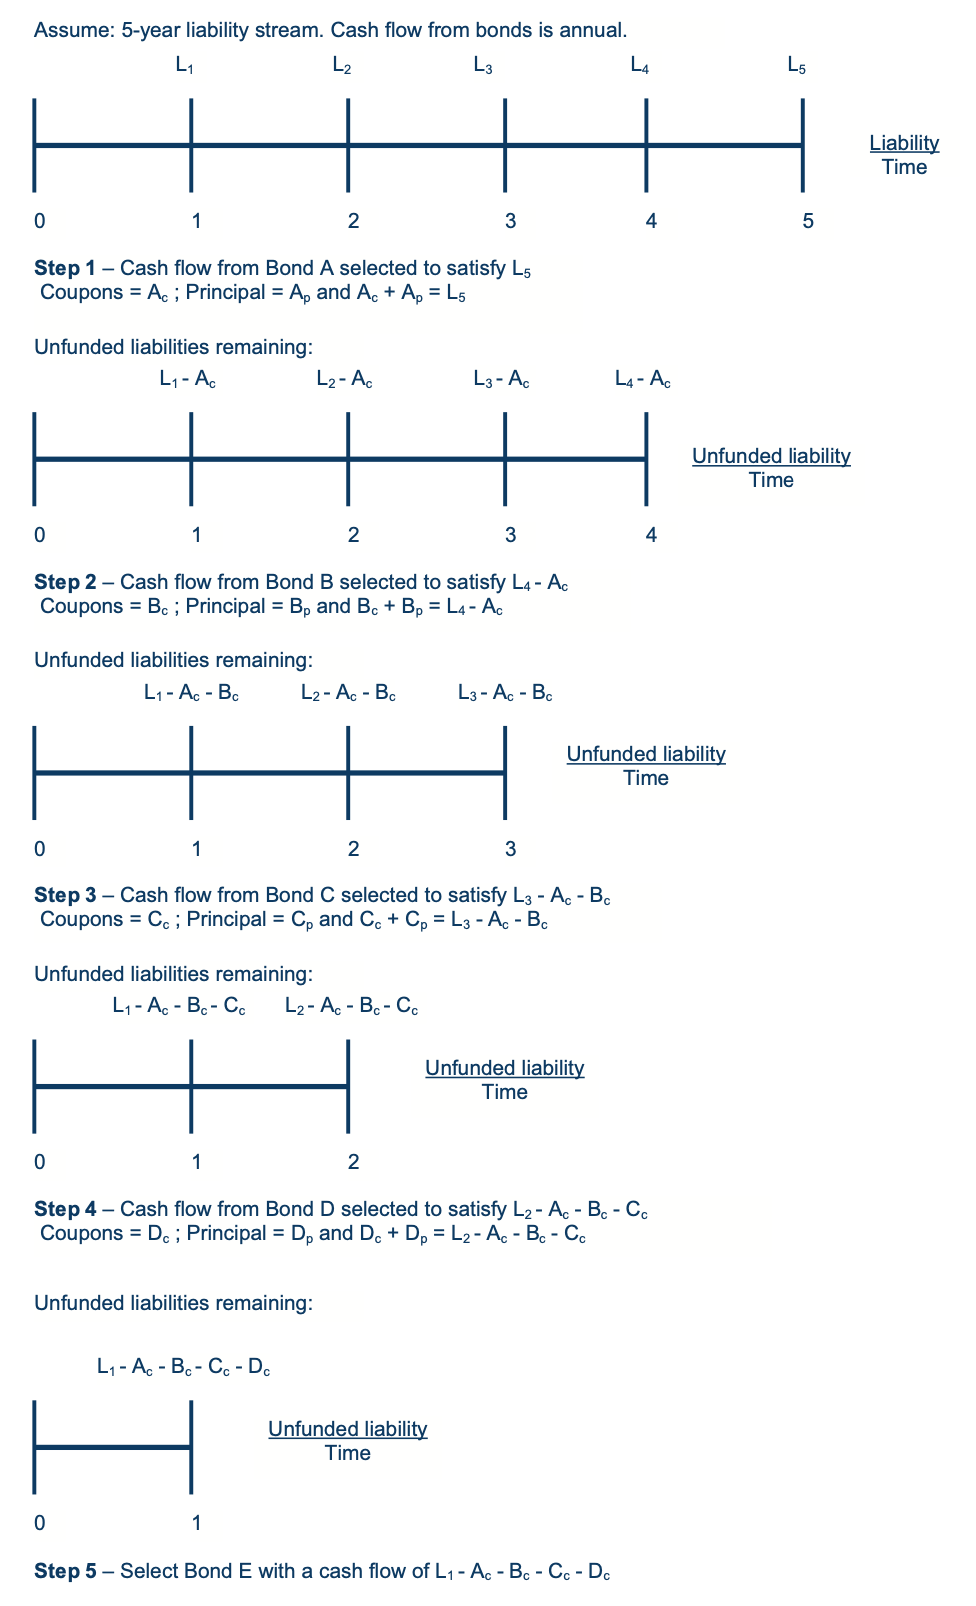
\includegraphics[width=14cm]{4}
\end{figure}

\section{Exemples}
\subsection{Question 1}
Le tableau ci-dessous présente le rendement actif sur six périodes d'un portefeuille obligataire. Calculez le portfolio’s tracking risk pour la période de six périodes.

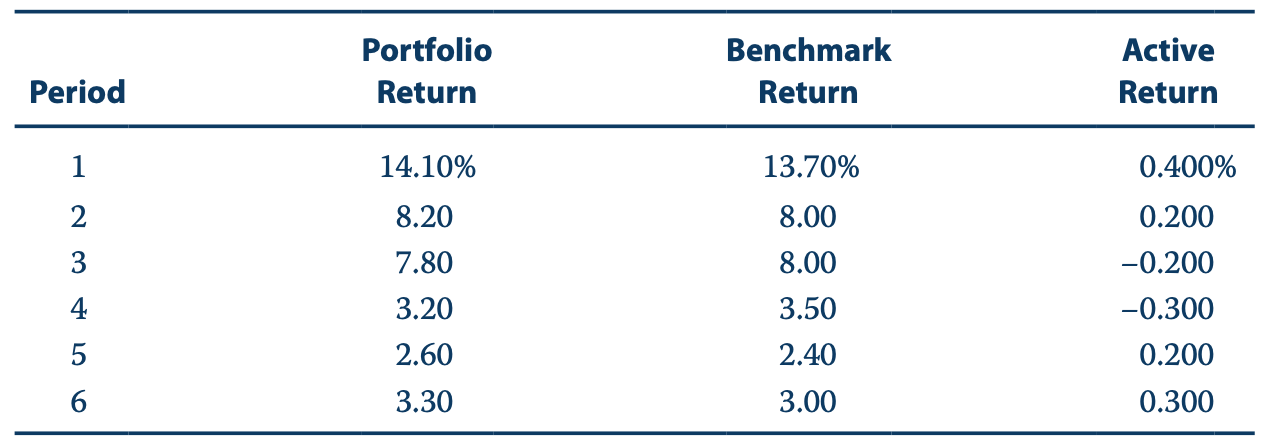
\includegraphics[width=14cm]{5}

\textbf{Le tracking risk est l'écart type des rendements actifs. Pour les données présentées dans le problème, le tracking risk  est de 28,284 point de base.}

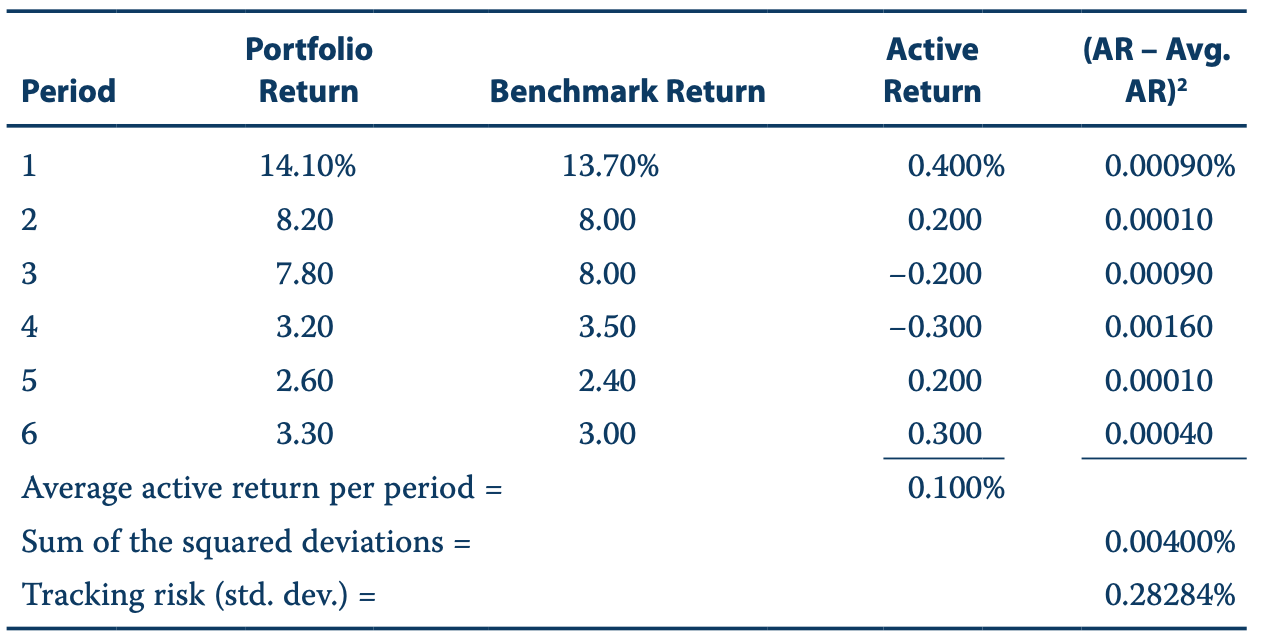
\includegraphics[width=14cm]{6}

\newpage

\subsection{Question 2}
Le tableau ci-dessous présente la duration du spread pour un portefeuille de 70 obligations et un indice de référence basé sur les secteurs. Déterminez si le portefeuille ou l'indice de référence est plus sensible aux variations du spread sectoriel en déterminant la duration du spread pour chacun. Compte tenu de votre réponse, quel est l’effet sur le portfolio’s tracking risk?

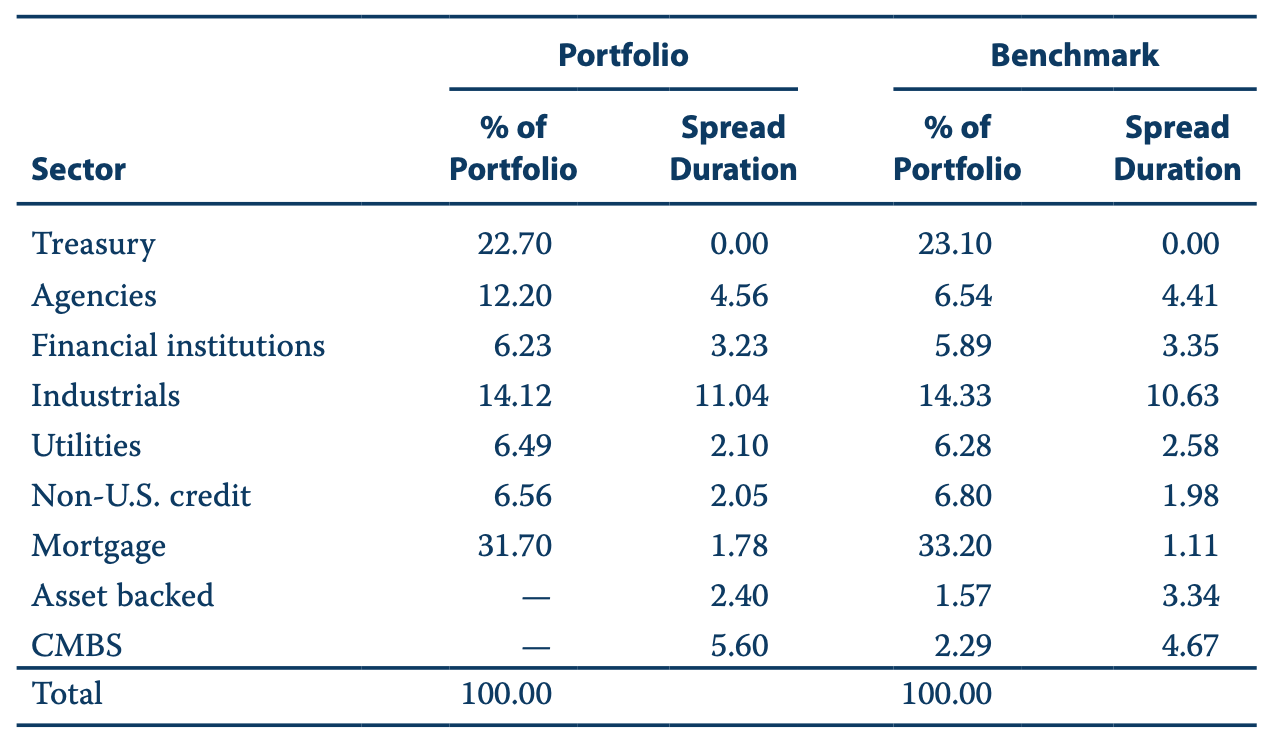
\includegraphics[width=14cm]{7}

\textbf{Le portefeuille est plus sensible aux variations du spread car sa duration du spread est de 3,151 par rapport à 2,834 de l’indice de référence. La durée plus élevée du spread du portefeuille est principalement attribuable au poids plus important du portefeuille sur les titres d’agence. La durée du spread pour chacun peut être calculée en prenant une moyenne pondérée des durées des différents secteurs. Puisqu'il existe une différence entre la duration du spread du portefeuille et celle de l'indice de référence,  le tracking risk sera plus élevé que si les deux étaient plus étroitement appariés.}

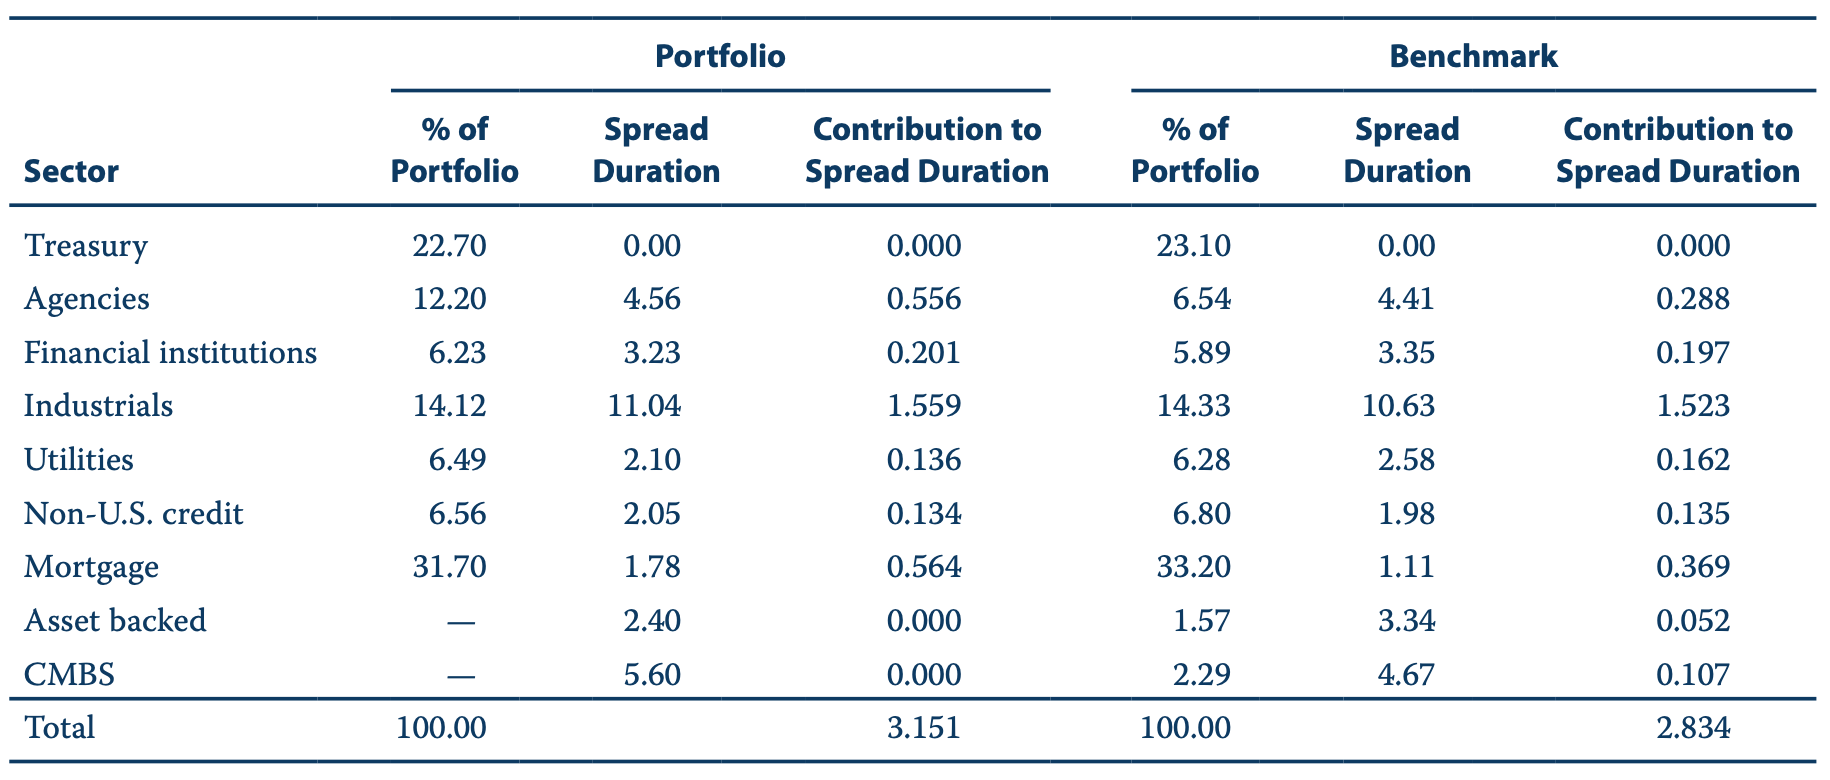
\includegraphics[width=16cm]{8}

\newpage

\subsection{Question 3}
Vous êtes le gestionnaire d'un portefeuille composé de trois obligations d'un montant nominal égal de 1 000 000 \$ chacune. Le premier tableau ci-dessous montre la valeur de marché des obligations et leurs durées. (Le prix comprend les intérêts courus.) Le deuxième tableau contient la valeur marchande des obligations et leur durée un an plus tard.

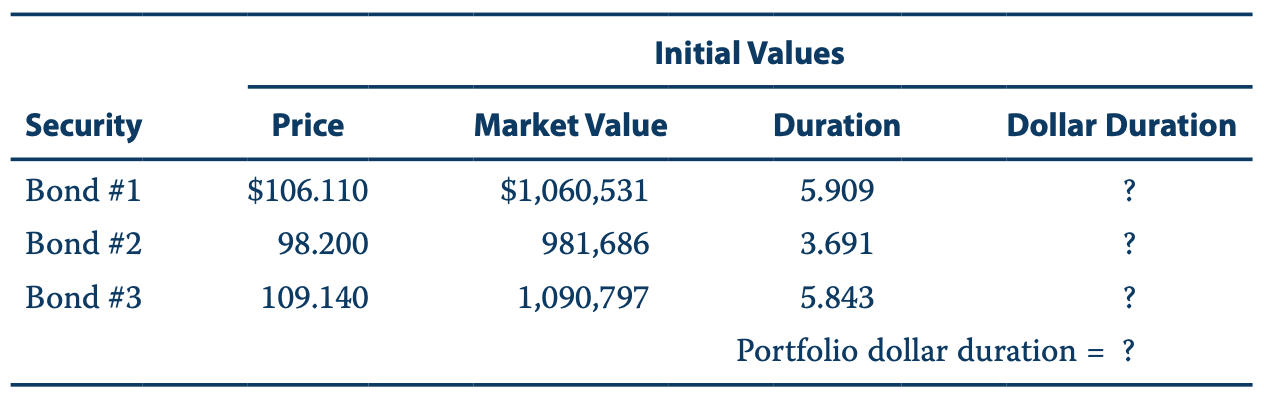
\includegraphics[width=14cm]{9}

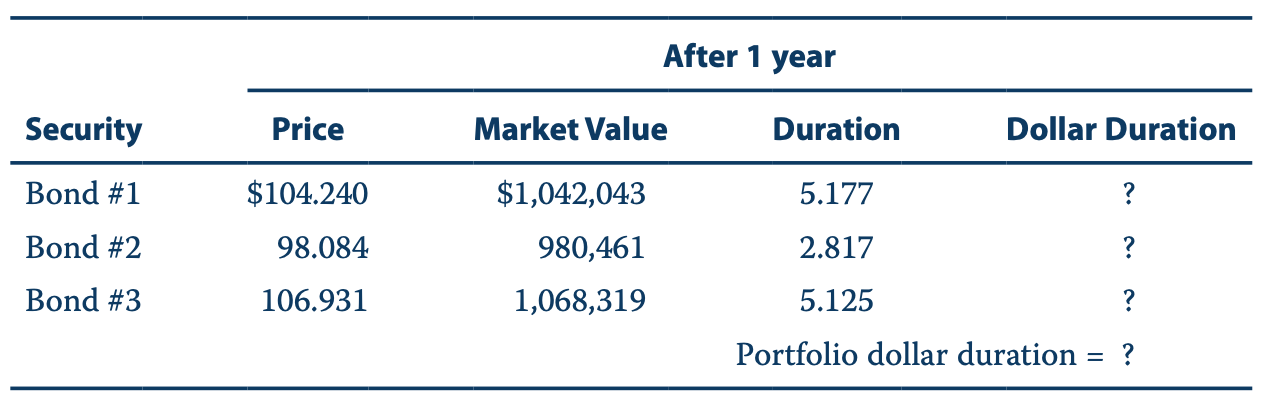
\includegraphics[width=14cm]{10}

En tant que gestionnaire, vous souhaitez maintenir la duration en dollars du portefeuille au niveau initial en rééquilibrant le portefeuille. Vous choisissez de rééquilibrer en utilisant les proportions de sécurité existantes d'un tiers chacune.  Calculer:
\begin{enumerate}
\item les durées en dollars de chacune des obligations.
\item le taux de rééquilibrage nécessaire au rééquilibrage.
\item les liquidités nécessaires au rééquilibrage.
\end{enumerate}

La duration en dollars est une mesure de la variation de la valeur du portefeuille pour une variation de 100 point de base des rendements du marché.  La duration en dollars d’un portefeuille est la somme des durées en dollars des titres qui le composent. La duration en dollars de ce portefeuille au début de la période est de 162636 \$.

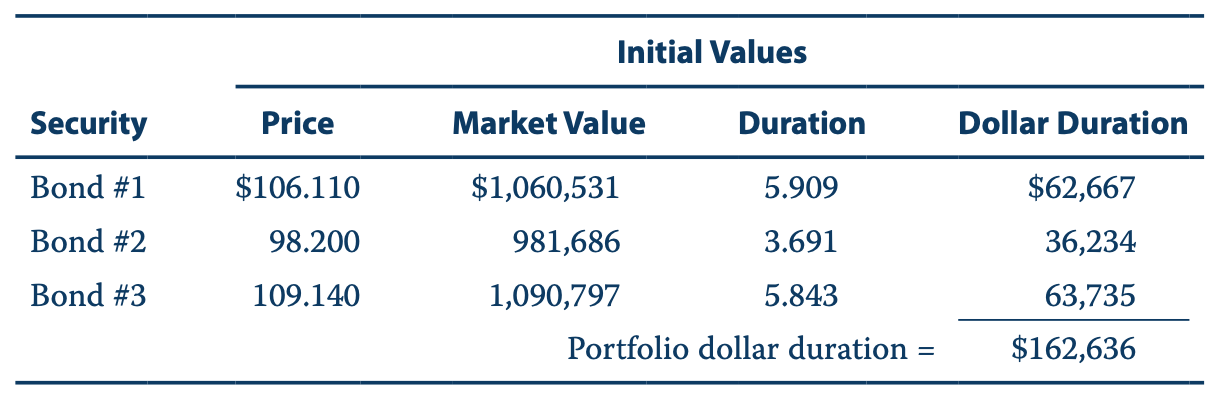
\includegraphics[width=14cm]{11}


À la fin d’un an, la duration en dollars du portefeuille est passée à 136 318 \$

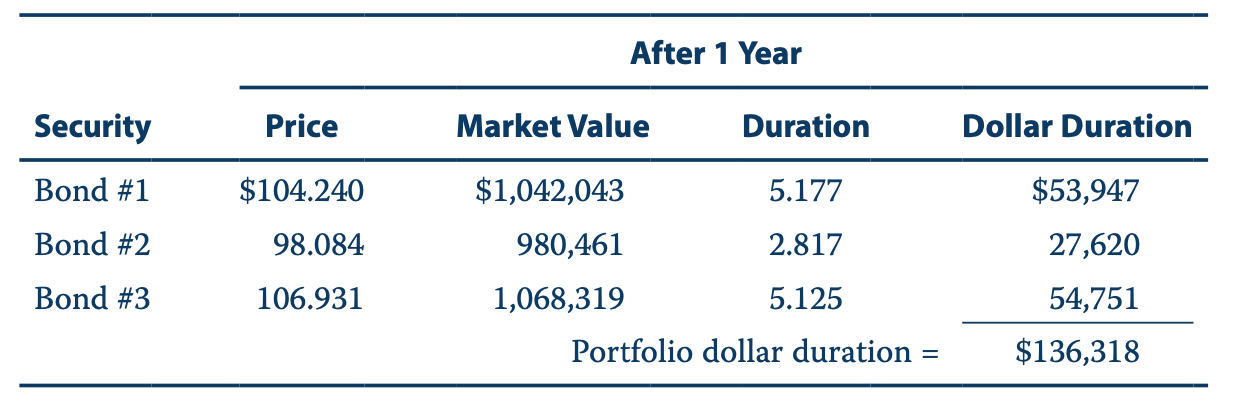
\includegraphics[width=14cm]{12}

Le ratio de rééquilibrage est un ratio de la durée d'origine en dollars sur la nouvelle durée en dollars:
\begin{align*}
\textbf{Rebalancing ratio} =\frac{162636}{136318} = 1.193
\end{align*}

Le portefeuille exige que chaque position soit augmentée de 19,3\%. La trésorerie nécessaire à ce rééquilibrage est calculée comme suit:

\begin{align*}
\textbf{Cash required} = 0.193 × (1042043 + 980461 + 1068319)=596529
\end{align*}

\newpage

\subsection{Question 4}
Le comité d'investissement de l'Université de Rojas est mécontent de la performance récente de la partie à revenu fixe de sa dotation et a licencié l'actuel gestionnaire de titres à revenu fixe. Le portefeuille actuel, comparé à l'indice Lehman Brothers U.S. Aggregate, est présenté dans le tableau suivant. Le comité d’investissement engage Alfredo Alonso, un consultant de MHC Consulting, pour évaluer les risques du portefeuille, soumettre des idées au comité et gérer le portefeuille de manière intérimaire.

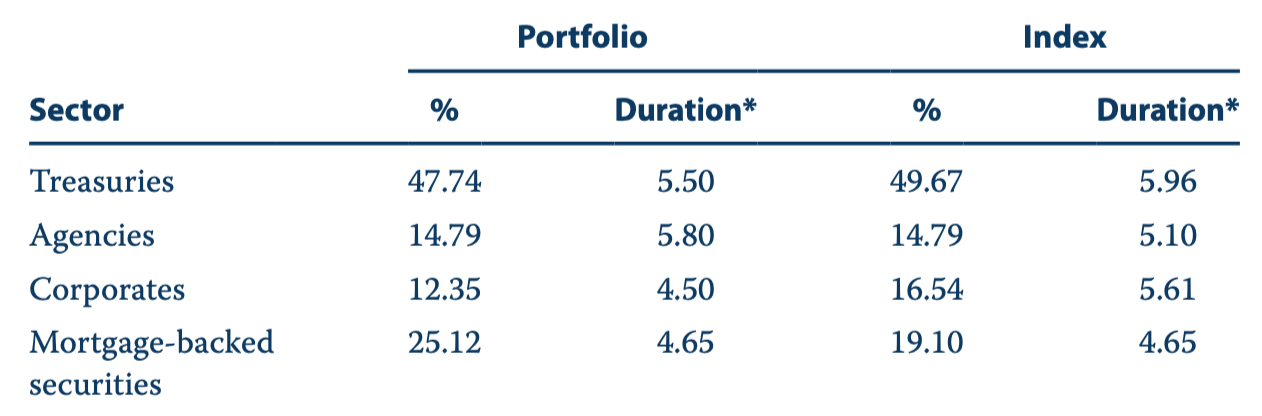
\includegraphics[width=14cm]{13}

Alonso remarque que le portefeuille du gestionnaire licencié ne détenait pas de titres en dehors de l’univers de l’indice. Le comité demande à Alonso d'envisager une stratégie d'indexation, y compris les avantages connexes et les problèmes logistiques. Alonso identifie trois facteurs qui limitent la capacité d'un gestionnaire à répliquer un indice obligataire:
\begin{enumerate}
\item Un manque de disponibilité de certaines émissions obligataires
\item Un manque de données indicielles disponibles pour positionner le portefeuille
\item Différences entre les prix des obligations utilisés par le gestionnaire et le fournisseur de l'indice
\end{enumerate}
Alonso a effectué une analyse plus approfondie de la portion actuelle du Trésor américain du portefeuille et a découvert une surpondération importante dans un bon du Trésor à 5 ans (valeur nominale de 10 millions de dollars). Il s'attend à ce que la courbe des taux s'aplatisse et prévoit un prix à l'horizon de six mois du bon du Trésor à 5 ans à 99,50 \$. Par conséquent, la stratégie d’Alonso consistera à vendre tous les bons du Trésor à 5 ans et à investir le produit dans des bons du Trésor à 10 ans et des liquidités tout en maintenant la duration en dollars du portefeuille. Les informations sur les obligations du Trésor américain sont présentées dans le tableau suivant:

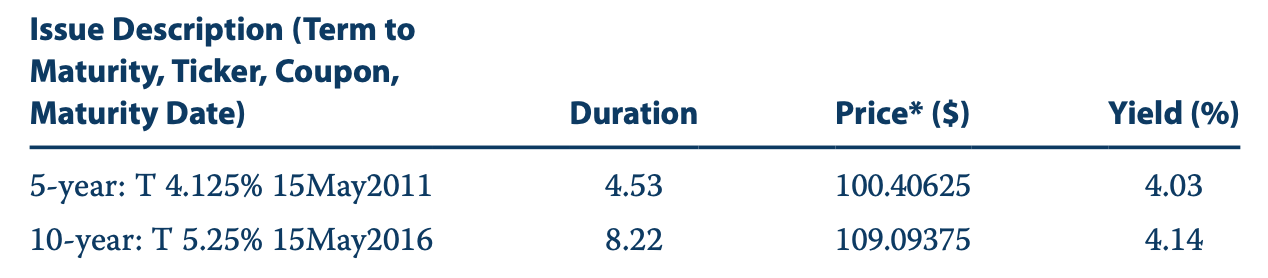
\includegraphics[width=14cm]{14}

\vspace{0.5cm}

\subsubsection*{Quelle est la durée du portefeuille de titres à revenu fixe de l'Université Rojas ?}
La durée du portefeuille est une moyenne pondérée des durées des obligations individuelles.
\begin{align*}
(0.4774 \times 5.50) + (0.1479 \times 5.80) + (0.1235 \times 4.50)+ (0.2512 \times 4.65) = 5.20735
\end{align*}

La durée du portefeuille est de 5.20735

\subsubsection*{Quelle est la stratégie de portefeuille obligataire utilisée par le gestionnaire licencié ?}
\begin{itemize}
\item Les pondérations du portefeuille diffèrent considérablement pour certains secteurs de celles de l'indice
\item Les durées des composantes du portefeuille diffèrent de leurs durées respectives dans l'indice.
\item Le gestionnaire utilise une gestion active car il permet un décalages de la durée et du secteur.
\end{itemize}

\subsubsection*{En ce qui concerne les trois facteurs identifiés par Alonso, quel est le facteur le moins susceptible de limiter la capacité d’un gestionnaire à répliquer un indice obligataire ?}
 Les données d'index sont facilement disponibles. Alonso a tort d'identifier cela comme un facteur limitant. Les informations (données) pour les deux autres facteurs peuvent être difficiles, voire impossibles à acquérir.
\subsubsection{Quelle est la valeur nominale des obligations à 10 ans à acheter pour exécuter la stratégie d’Alonso ?}
Alonso ne va pas simplement réinvestir l'intégralité du produit de la vente dans des bons du Trésor à 10 ans, car son désir déclaré est de maintenir la duration en dollars du portefeuille. Le prix de vente de 10 millions de dollars de la valeur nominale de l'obligation de 5 ans est obtenu en multipliant $10000000 \times 1.0040625 = 10040625$ . La durée en dollars de la période de 5 ans est de $4,53 \times 10040625 \times 0.01 = 454840.31$ . Divisez maintenant 454 840.31  par le produit de la durée du 10 ans et de son prix coté et 0.01 pour obtenir la valeur nominale du 10 ans. Le résultat est $454840.31  / (8,22 \times 1,0909375 \times 0.01) = 5072094$.
\end{document}